\documentclass[11pt]{article}

\usepackage[utf8]{inputenc}
\usepackage[margin=2cm]{geometry}
\usepackage{cite}
\usepackage{natbib}
\usepackage{bibentry}
\usepackage{hyperref}
\usepackage{outlines}
\usepackage{enumitem}
\usepackage{graphicx}
\usepackage[utf8]{inputenc}

%\setenumerate[1]{label=\Roman*.}
%\setenumerate[2]{label=\Alph*.}
%\setenumerate[3]{label=\roman*.}
%\setenumerate[4]{label=\alph*.}

\nobibliography*
	
\begin{document}
	
	\title{An Introduction to Egyptian Hieroglyphs -- CRN 11077}
	\author{C. Casey \\
		Wilbour Hall 302 \\
  		\texttt{\href{mailto:christian_casey@brown.edu}{christian\_casey@brown.edu}}}
	\date{\today}
	\maketitle
	
	\section*{Class Meeting Time/Place}
	
		\begin{tabular}{l l}
		Date: & July 17 - July 21, 2017 \\
		Time: & 9:00 - 11:50 \\
		Place: & J. Walter Wilson 403
		\end{tabular} 
		
% Description		
	\section*{Learn Ancient Egyptian!}
		
		Starting next week, you will have the opportunity to participate in a free Summer@Brown course on Ancient Egyptian.
		We will do a number of fun activities together and learn a lot in the process. 
		You will even get to create your own hieroglyphic text (Fig. \ref{figPapyrus}) and go on a field trip to Brown's museum storage, where we will read a real, 3000-year-old Egyptian papyrus, never before seen by the public.
		
		In this class, you will learn: 
			how to read write Egyptian Hieroglyphs, 
			the history of the Egyptian language, 
			a ton of vocabulary, 
			and the basics of Egyptian syntax.
		
		\begin{figure}[!h]
		\centering
		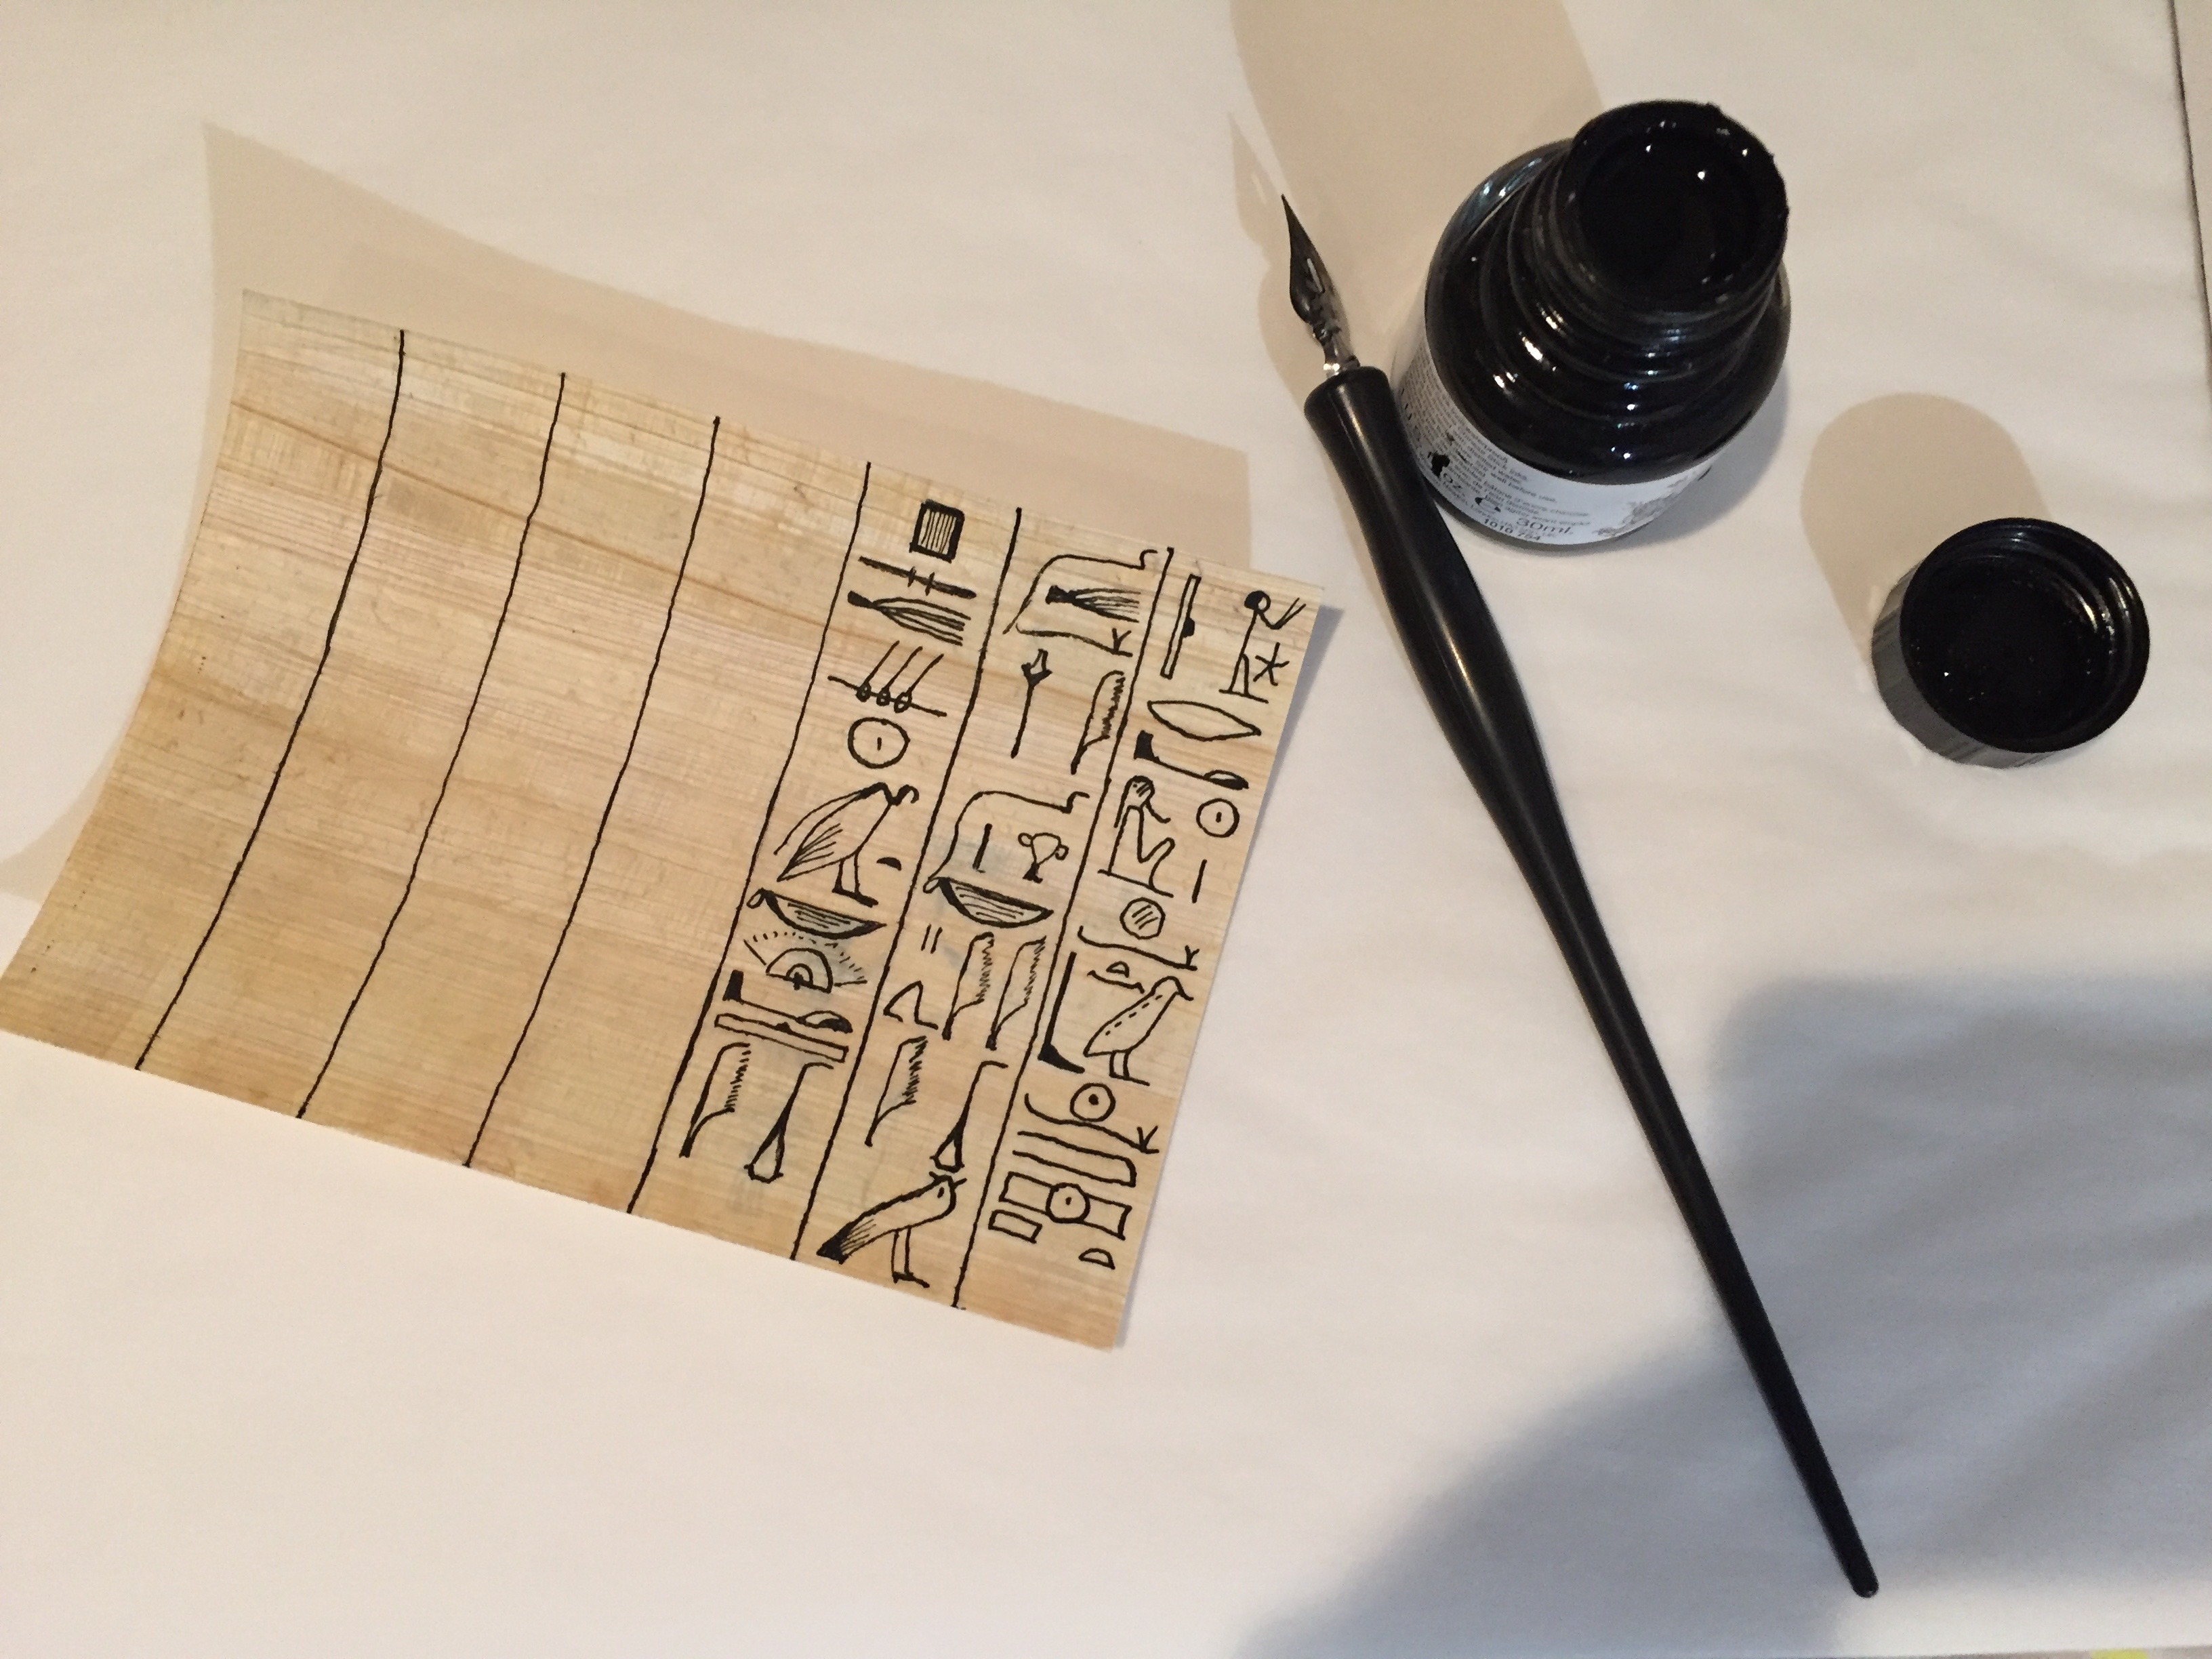
\includegraphics[scale=0.05]{cursive}
		\caption{For the final project, you will create your own hieroglyphic text on papyrus.}
		\label{figPapyrus}
		\end{figure}
		
	\section*{Be part of an important research project}
		
		By participating in the class, you will become part of an ongoing experiment.
		In order to test a question about language pedagogy, I will teach two slightly different classes, one to a group of volunteers (you) and one to the students enrolled in the regular Summer@Brown course. 
		This means that your class will differ from the regulary (paid) course in one small way, but it will otherwise be exactly the same.
		Your scores and evaluations will be collected for this study, but you will be entirely anonymous (even to me).
		There are only five spaces available. They will be given to the first students who send me an email at the address listed above.
		

\end{document}













